\documentclass[]{auvsi_doc}
\setkeys{auvsi_doc.cls}{
	AUVSITitle={Failure Modes and Effects Analysis},
	AUVSIRevision=0.0,
	AUVSIDescription={Created},
	AUVSIAuthor={Kameron Eves},
	AUVSIChecker={[Checker]},
	AUVSILogoPath={./figs/logo.pdf},
	AUVSIDocID={AF-004}
}

% include extra packages, if needed

\begin{document}

\begin{AUVSITitlePage}
\begin{artifacttable}
\entry{AF-007, 0.1, 02-19-19, Initial creation, Kameron Eves, Tyler Critchfield}
\entry{AF-007, 1.1, 04-05-19, Updated After System Refinement, Kameron Eves, Andrew Torgesen}
% additional \entry{} commands for extra rows in the revision table, if needed
\end{artifacttable}
\end{AUVSITitlePage}
\vspace*{-2cm}
% document contents (see below for LaTex commands that make your life easier)
\section{Introduction}
\vspace*{-0.5cm}
To mitigate risk of failure within the competition, a Failure Modes and Effects Analysis (FMEA) was performed. Many deficiencies were found and were then corrected to an acceptable level.
\vspace*{-0.5cm}
\section{Analysis}
\vspace*{-0.5cm}
\hspace*{-1.54cm}
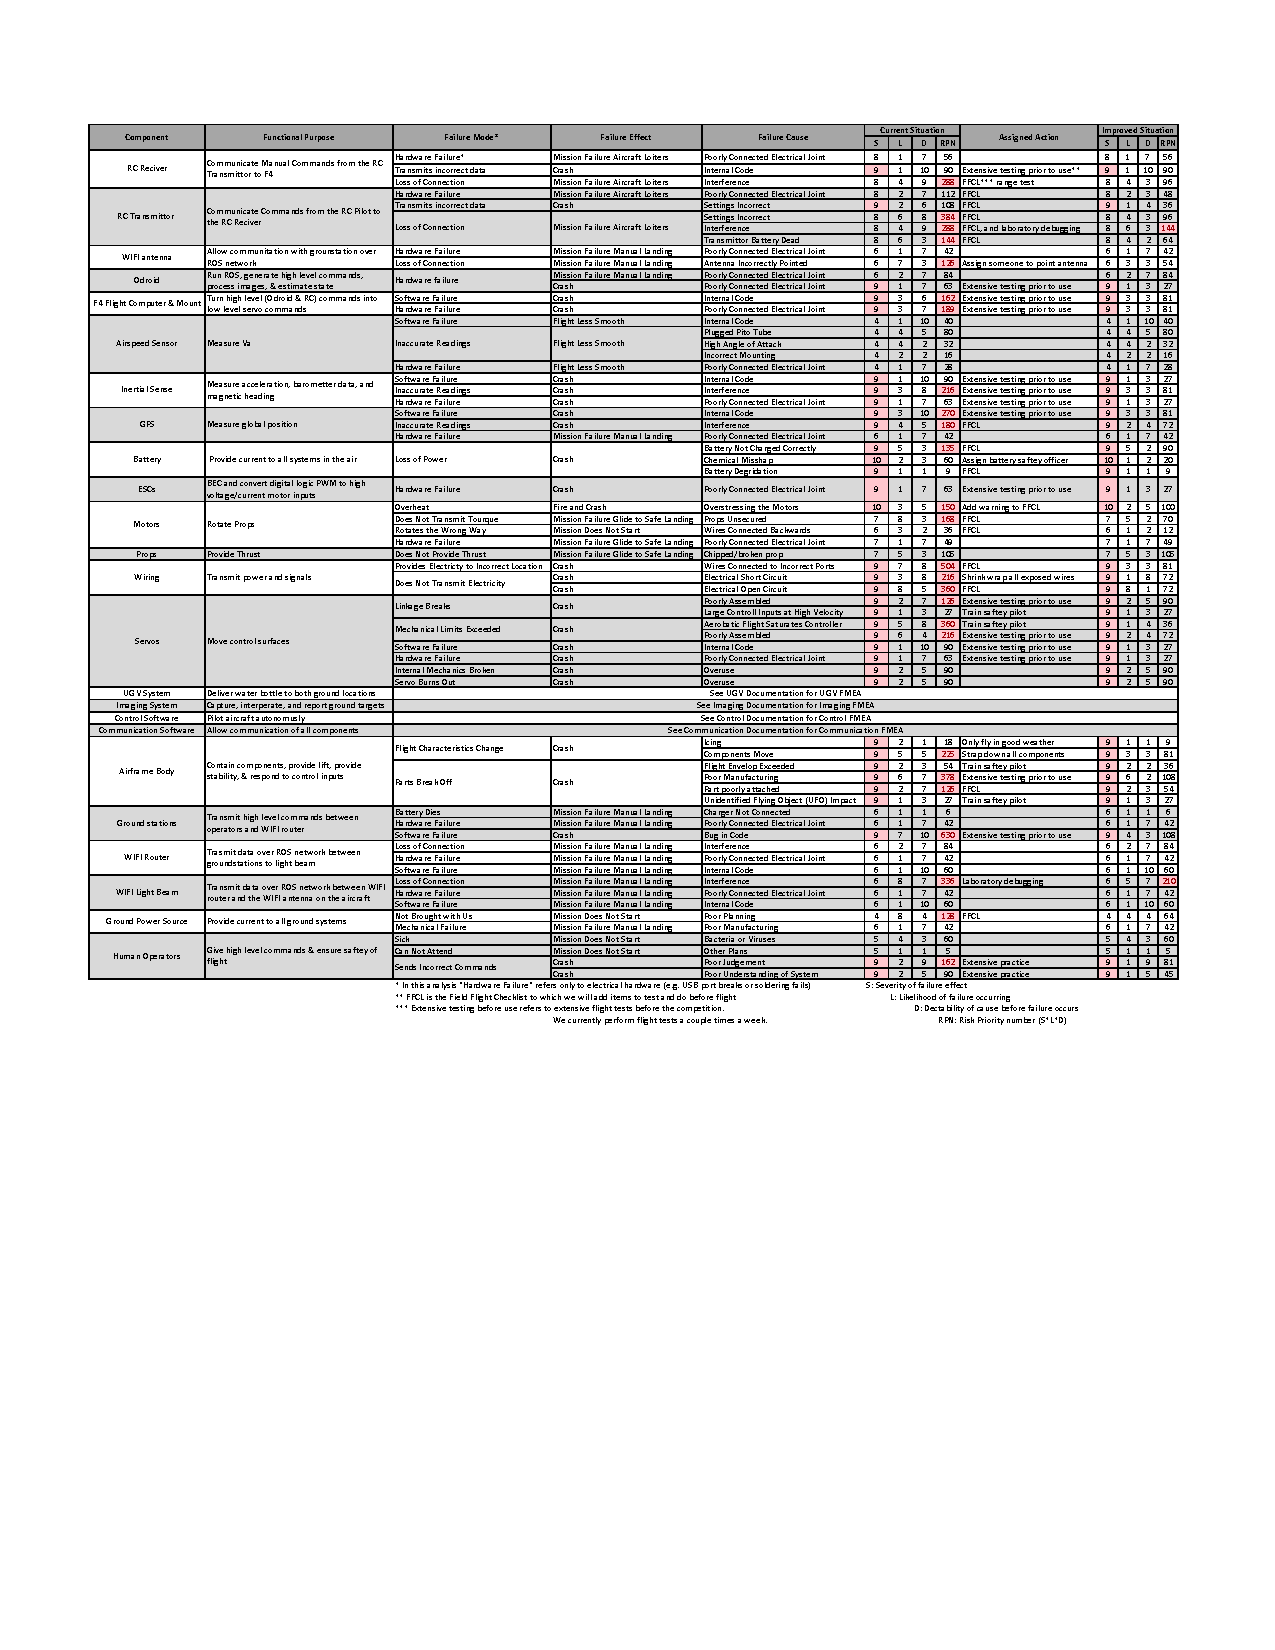
\includegraphics[width=1.2\textwidth]{./figs/FMEA.pdf}
\label{fig:reqMat}

\section{Discussion}
As can be seen from this analysis, most of the concerning issues were addressed. We are now confident in our ability to fly a failure free mission with the exception of one issue: we continue to see communication drop out for a couple systems. We do not completely understand why this is happening. It seems to be somewhat location dependent and occurs randomly. It does not usually affect our missions, but its risk priority number (RPN) is high enough that we wanted to address it. We have since performed tests in several locations to see if we can identify the root cause and solution to these communication issues. We have found that the GPS drop out issues occur less frequently than previously expected. As such, its RPN is within acceptable levels. We are still experiencing communication drop in the remote control signal and the WIFI signal. We would like to be confident that this issue will not arise at the competition and so are performing laboratory testing to find a way to fix these issues.




\end{document}
